
\documentclass[10pt, conference, compsocconf]{IEEEtran}

% Packages
\usepackage[pdftex]{graphicx}

% for tables (use if required!)
\usepackage{setspace}
\usepackage{longtable}
\usepackage{colortbl}
\usepackage{array}
\usepackage{ragged2e}
\usepackage{lscape}
\usepackage{tabularx}
\usepackage{multirow}
\usepackage{booktabs}
\usepackage{url} 

%Anpassung der Namen f\"ur Abbildung und Tabelle
\usepackage[figurename={Abbildung},tablename={Tabelle}]{caption}

% Better handling of floats
\usepackage{float}

\newcolumntype{w}[1]{>{\raggedleft\hspace{0pt}}p{#1}}
\newcolumntype{x}[1]{>{\centering\hspace{0pt}}p{#1}}


% Set spaces between and after floats here:
\setlength{\textfloatsep}{8pt} % Vertical space below (above) [t] ([b]) floats


\newcommand{\conforms}{\mathrel{\widehat{=}}}


% correct bad hyphenation here
\hyphenation{}


% correct bad hyphenation here
\hyphenation{op-tical net-works semi-conduc-tor}


\begin{document}
\title{Entwicklung einer Einkaufslisten-App}


\author{\IEEEauthorblockN{Markus H\"ul\ss}
\IEEEauthorblockA{
E-Mail: huma1200@stud.hs-coburg.de}
\\
\IEEEauthorblockN{Tanja M\"ogn}
\IEEEauthorblockA{
E-Mail: mota1200@stud.hs-coburg.de}
\and
\IEEEauthorblockN{Malcolm K\"ogler}
\IEEEauthorblockA{
E-Mail: koma1200@stud.hs-coburg.de}
\\
\IEEEauthorblockN{Daniel M\"uller}
\IEEEauthorblockA{
E-Mail: muda1200@stud.hs-coburg.de}
}

% make the title area
\maketitle


\begin{abstract}
Mangels Verf\"ugbarkeit von multiplattformf\"ahigen Apps zur Verwaltung von Einkaufslisten entstand die Idee, eine solche App zu entwickeln. Um den Entwicklungsaufwand m\"oglichst gering zu halten und nicht f\"ur jede Plattform separat eine App zu programmieren, entschieden wir uns f\"ur das Framework Phonegap. Dieses Paper besch\"aftigt sich mit der Konzeption und Entwicklung der App.   
\end{abstract}

\IEEEpeerreviewmaketitle

\section{Einleitung}
% no \IEEEPARstart
Immer pr\"asent und nicht mehr aus dem Alltag wegzudenken, unterst\"utzt  uns das Smartphone heute schon bei der Organisation und Kommunikation. Vor einigen Jahren hat man vor dem Einkauf noch schnell einen Einkaufszettel geschrieben. Aber wie schnell war der Zettel doch in der Tasche spurlos verschwunden, obwohl man sich so sicher war, ihn eingepackt zu haben. Heutzutage bietet sich das Smartphone als M\"oglichkeit an, einen Einkaufszettel zu speichern. Das bietet unter anderem die M\"oglichkeit, den Einkaufszettel zu jeder Zeit zu erweitern oder ihn mit anderen zu teilen. 
Ziel dieser Arbeit ist es, eine App zur Verwaltung von Einkaufszetteln zu entwickeln.
Diese soll es erm\"oglichen, erstellte Einkaufszettel mit anderen zu teilen.
Die jeweilige Plattform des App-Benutzers sollte dabei kein Hindernis darstellen.
Die Projektgruppe wurde in zwei Teams aufgeteilt. 
Ein Team war f\"ur die Frontend-Entwicklung zust\"andig, das andere f\"ur das Backend. 
Der Programmcode wurde mittels des Versionierungssystems GIT verwaltet. 
Grafiken wurden mit Balsamiq und MS Visio 2013 erstellt. 
Die Kommunikation erfolgte teils pers\"onlich, teils \"uber E-Mails.

Am Anfang wurde eine Konkurrenzanalyse angefertigt, um einen \"Uberblick \"uber die bereits am Markt verf\"ugbaren Apps zu erm\"oglichen.
Als N\"achstes wird die Erstellung von Prototypen anhand von Mockups beschrieben, welche die Grundlage f\"ur die Entwicklung bildeten.
Darauf folgend werden die verwendeten Technologien in Frontend und Backend im Zusammehang mit dem Nutzen in der App vorgestellt. Zuletzt werden in einer Zusammenfassung die Projekterfolge und Misserfolge aufgezeigt.

\section{Konkurrenzanalyse}
Um sich einen \"Uberblick \"uber vorhandene Apps zu verschaffen, wurde eine Konkurrenzanalyse erstellt.
Diese Konkurrenzanalyse beschr\"ankt sich auf native Apps und l\"asst Cloud-basierte L\"osungen au{\ss}en vor.
Zu diesem Zweck wurden die Top-Apps aus den App-Stores f\"ur die Plattformen Android, IOS und Windows Phone miteinander verglichen.
Um die Apps miteinander vergleichen zu k\"onnen, wurden drei Merkmale definiert. 
Diese Merkmale waren Plattformunabh\"angigkeit bzw. Multiplattformf\"ahigkeit, 
die M\"oglichkeit, Einkaufslisten mit anderen Leuten zu teilen sowie eine zentrale Datenhaltung mit Sychronisierung der Daten \"uber mehrere Ger\"ate hinweg.

Am Markt gibt es mittlerweile mehrere Apps, die darauf spezialisiert sind, Einkaufslisten zu verwalten.
Nur eine App bietet eine native Implementierung f\"ur die oben genannten Plattformen. Einige Apps bieten eine reduzierte Multiplattformf\"ahigkeit in dem Sinne, dass ein Webservice zu Verf\"ugung gestellt wird, \"uber den auf die Daten zugegriffen werden kann.
Die meisten Apps bieten ein Backbone zur zentralen Datenhaltung.
Nur wenige Apps bieten die M\"oglichkeit, Einkaufslisten mit anderen zu teilen. Diese F\"ahigkeit ist teilweise darauf beschr\"ank,t eine Einkaufsliste per E-Mail zu 
verschicken.

\section{Mockups}
Zu Beginn der Entwicklung wurde eine M\"oglichkeit gesucht, schnell einen Prototypen der App zu entwickeln.
Zu diesem Zweck wurden Mockups f\"ur das Frontend erstellt. 
Diese wurden in Teamarbeit entworfen und somit hatte jeder im Team eine Vorstellung, wie die App sp\"ater aussehen soll.
\begin{figure}[h!]
	\centering
	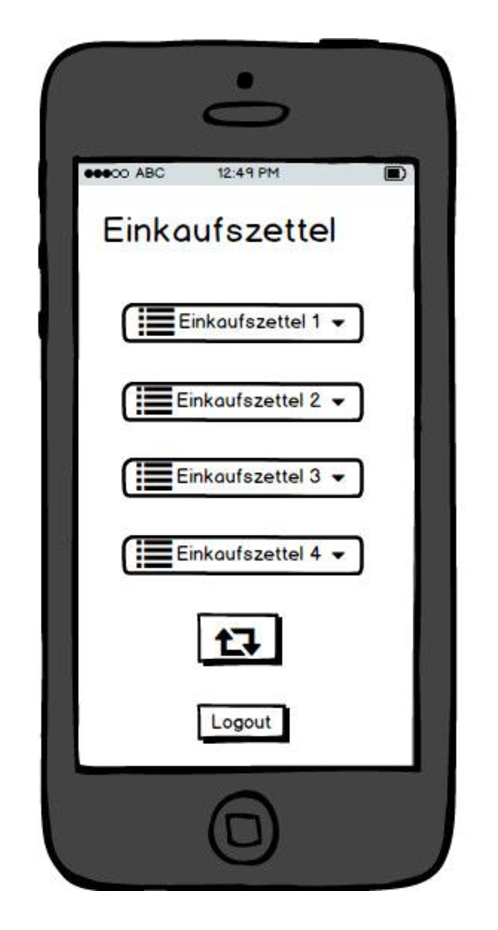
\includegraphics[scale=0.3]{./Bilder_Zeichnungen/Uebersicht.pdf}
	\caption{Einzelansicht}
	\label{fig:Mockup_Einzelansicht}
\end{figure}
In Abbildung~\ref{fig:Mockup_Einzelansicht} ist ein Beispiel f\"ur ein solches Mockup zu sehen. Die Abbildung~\ref{fig:Mockup_Einzelansicht} zeigt die Ansicht eines Einkaufszettels mit den zugeh\"origen Steuerelementen.

\section{Frontend}
Ein wichtiges Ziel ist es, eine plattform- und aufl\"osungsunabh\"angige Darstellung zu erm\"oglichen. 
Dabei soll das Frontend nicht f\"ur jede Plattform separat entwickelt werden.
Dies soll sowohl den Zeitaufwand als auch potenzielle Fehlerquellen verringern. 
Der Browser dient als Grundlage f\"ur die Darstellung. 
Somit ist eine einfache Darstellung auf mobilen Ger\"aten und Desktop-PCs m\"oglich.
Dieser Abschnitt befasst sich mit den beiden Komponenten "Phonegap" und "jQuery mobile".

\subsection{Phonegap}
Die auf dem Markt vorhandenen Applikationen entwickeln f\"ur Android, iPhone und Windows Phone jeweils se\-parate native Apps. 
Das erfordert tiefgehendes Know-how f\"ur die einzelnen Plattformen und weitergehende separate Behandlung von Fehler- und Change-Requests. 
Aus diesem Grund wird bei der Entwicklung der App auf Phonegap gesetzt. Phonegap ist ein Framework zum Erstellen von nativen Anwendungen f\"ur die g\"angigsten mobilen Plattformen durch die Verwendung von HTML5.
Das Konzept von Phonegap ist, auf einer Seite das Frontend einer Anwendung \"uber eine angezeigte Webseite im Browser zu realiseren. 
Auf der anderen Seite stellt es zus\"atzlich Javasript API's bereit, die einem Zugriff auf bestimmte Hardware wie die Kamera oder bestimmte Sensoren erm\"oglichen. 
Auch kann auf Events wie beispielsweise eine schwache Funkverbindung reagiert werden. 
Somit sind Funktionalit\"aten nativer Apps gegeben, ohne sich intensiv mit der Architektur jeglicher Zielplattformen auseinanderzusetzen.
Zus\"atzlich baut Phonegap am Ende aus diesen Komponenten eine native App, welche sich in dem dementsprechenden Store anbieten l\"asst.

\subsection{jQuery Mobile}
Ein zus\"atzliches Problem neben den unterschiedlichen Plattformen, ist die Vielzahl an unterschiedlichen Browsern und Displayaufl\"osungen der Endger\"ate. 
Die Anwendung soll ein einheitliches Design, unabh\"angig von Browser und Aufl\"osung besitzen. 
Ein Benutzer soll sich nicht bei einem Wechseln zwischen einem normalen und einem mobilen Browser bei der Bedienung umgew\"ohnen m\"ussen. 
Um dieser Anforderung nachzukommen, wird auf das jQuery Mobile Framework zur\"uckgegriffen.
Es erm\"oglicht eine einfache Umsetzung von Webseiten mit einem responsive Design und bietet eine gro{\ss}e Auswahl unterst\"utzter Browser (sowohl mobile als auch non-mobile). 
Somit wird mit einer einzigen Version des Frontends eine gro{\ss}e Menge an Endger\"aten unterst\"utzt und dies tr\"agt zu einer schnellen Entwicklung der Anwendung bei. 
Zus\"atzlich ist es mit dem Multi-Page-Layout-Konzept m\"oglich, mit einer einzigen HTML-Seite alle Ansichten einer App darzustellen. Dadurch muss nicht bei jedem Wechsel einer Ansicht eine neue Seite heruntergeladen werden, womit sich die Performance verbessert und Traffic gespart wird. (Bisherige Quelle bisher nur die jQuery Mobile-Website)

\section{Backend}
Ein weiteres wichtiges Ziel ist es, eine endger\"ateunabh\"angige Datenspeicherung zu gew\"ahrleisten. 
Daf\"ur ist ein Backend, das von \"uberall \"uber das Internet zu erreichen ist, vonn\"oten. 
F\"ur die Umsetzung des Projekts entschieden wir uns f\"ur einen einfachen Webserver und die Nutzung von PHP und MySQL zur Datenhaltung und f\"ur JSON nach dem ReST-Standard zur Kommunikation zwischen Anwendung und Backend.  
Dieser Abschnitt befasst sich mit den Komponenten PHP, MySQL und JSON, welche die Umsetzung der Anforderungen erm\"oglichen.

\subsection{PHP}
PHP wird im Backend verwendet, um die Schnittstelle zwischen Anwendung und Datenbank auf dem Webserver zu stellen. PHP unterst\"utzt unz\"ahlige Datenbanktypen und ein breites Spektrum an Funktionalit\"aten zur Konvertierung in das JSON-Format.

\subsection{MySQL}
MySQL ist ein weit verbreitetes relationales Datenbanksystem und kam vor allem wegen seiner Platt\-formunabh\"angigkeit und der kostenfreien Nutzung unter der OpenSource-Lizenz zur Umsetzung der Datenbank in Frage. 
Bei der Auswahl spielte auch die M\"oglichkeit der Verwendung von verschiedenen Speicherssubsystemen eine Rolle. 
Durch die Verwendung von InnoDB stehen Rollback und Transaktionssicherungsm\"oglichkeiten zur Verf\"ugung, dies ist ein wichtiger Gesichtspunkt im Bezug auf Datensicherheit.

\begin{figure*}[t]
	\centering
	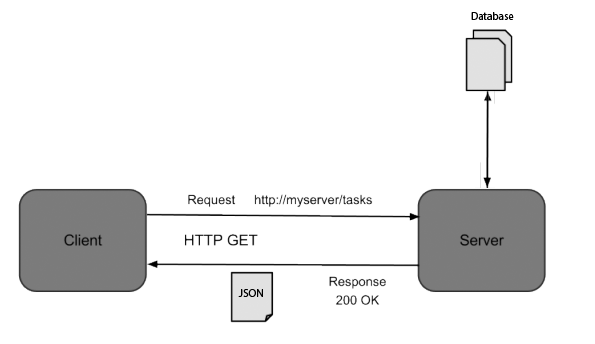
\includegraphics[width=0.8\textwidth]{./Bilder_Zeichnungen/Architektur_2.png}
	\caption{3-Wege-Architektur f\"ur die App}
	\label{fig:Architektur}
\end{figure*}

\subsection{JSON}
Aufgrund der Verwendung des auf Javascript basierenden Frameworks JQuery-Mobile zur Erstellung einer Webapp lag die Verwendung von JSON als Format zum Datenaustausch zwischen Anwendung und Backend nahe. 
Dadurch ist es m\"oglich, die Daten vom Backend ohne vorherige Konvertierung in der Anwendung zu verwenden. 
Mithilfe von PHP l\"asst sich so die Schnittstelle nach dem ReST-Programmierparadigma gestalten,welche die geforderten Daten im JSON zur\"uckliefert. 

\section{Architektur}
{Damit die einzelnen Komponenten ordnungsgem\"a{\ss} so zusammenarbeiten, ben\"otigt es noch einer passenden Architektur. Aufgrund der verwendeten Technologien wird eine Drei-Schichten-Architektur verwendet. Somit l\"asst sich eine Trennung von Pr\"asentation und Anwendungslogik realisieren.
	
Die Abbildung~\ref{fig:Architektur} zeigt den genauen Aufbau der Architektur. Ein Client sendet seine Aktion per HTTP-Request an den Webserver. Dieser holt geforderte Daten aus der Datenbank oder \"andert diese. Die von der Datenbank erhaltenen Daten werden in das JSON-Format konvertiert. Danach werden sie als Inhalt des HTTP-Response an den Client gesendet. Der genauere Ablauf ist im Abbildung~\ref{fig:Sequenzdiagramm} ersichtlich.

\begin{figure}[h!]
	\centering
	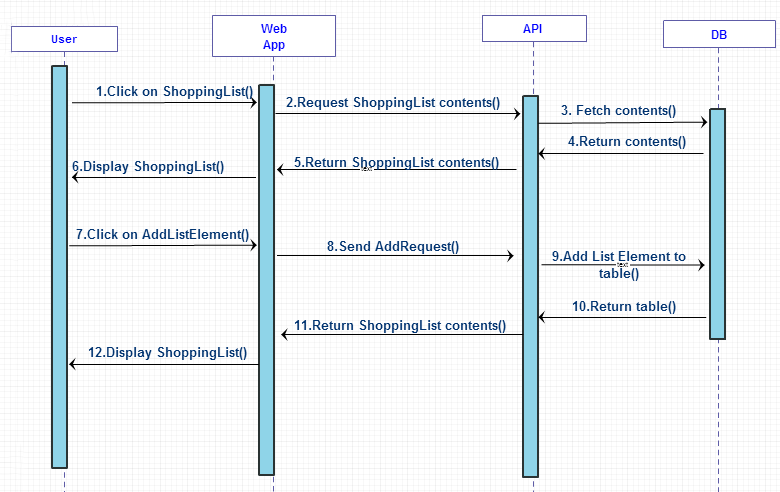
\includegraphics[width=0.45\textwidth]{./Bilder_Zeichnungen/Sequenzdiagramm.png}
	\caption{Sequenzdiagramm}
	\label{fig:Sequenzdiagramm}
\end{figure}

\section{Fazit}
Die Verwendung des Phonegap Frameworks brachte den Vorteil, dass ohne gro{\ss}e R\"ucksicht auf die Plattform entwickelt werden konnte. 
Der Einsatz von JQuery mobile erm\"oglicht eine einheitliche Darstellung der mobilen Web-App auf allen Ger\"aten.
Die Einbindung von anderen Frameworks war mit Komplikationen verbunden.
Da viele Javascript-Frameworks den DOM-Tree manipulieren, gestaltet sich ein gleichzeitiger Einsatz mehrerer Javascript-Frameworks als schwierig.


\section {Ausblick}
Die App besitzt bereits alle notwendigen Funktionen, um eine Einkaufsliste zu erstellen, zu editieren und zu teilen. In der weiteren Entwicklung zeigen sich die Vorteile, die von Phonegap geboten werden. 
So kann beispielsweise ein Offline-Modus entwickelt werden, der es erm\"oglichen soll, die App auch ohne permanente Internetverbindung zu nutzten. 
%Das ist mit Phonegap m\"oglich, da man mit diesem Framework die Qualit\"at der Internetverbindung abfragen kann. 
Des Weiteren ist an eine intelligentere Unterst\"utzung der App im Alltag gedacht. 
Die App soll beispielsweise den User benachrichtigen, falls ein anderer User in einer gemeinsamen Einkaufsliste einen Eintrag ge\"andert oder hinzugef\"ugt hat. 
%Hier ist wichtig das unbedingt der native Benachrichtigungsmodus des Systems verwendet wird um so viel Usability wie m\"oglich zu %gew\"ahrleisten. 
Ein weitere Verbesserung w\"are auch die permanente Lokalisierung des Users und eine Reaktion der Einkaufslisten-App, wenn sich der User in der N\"ahe oder in einem Einkaufsladen befindet. 


\end{document}


